\documentclass{article}
\usepackage[utf8]{inputenc}
\usepackage{geometry}
 \geometry{
 a4paper,
 total={170mm,257mm},
 left=20mm,
 top=20mm,
 }
 \usepackage{graphicx}
 \usepackage{titling}

 \title{Lab 4: Clustering }
\author{Yadder Aceituno}
\date{October 2025}
 
 \usepackage{fancyhdr}
\fancypagestyle{plain}{%  the preset of fancyhdr 
    \fancyhf{} % clear all header and footer fields
    \fancyfoot[R]{
\includegraphics[width=2cm]{images/um.png}}
    \fancyfoot[L]{\thedate}
    \fancyhead[L]{Data Mining}
    \fancyhead[R]{\theauthor}
}
\makeatletter
\def\@maketitle{%
  \newpage
  \null
  \vskip 1em%
  \begin{center}%
  \let \footnote \thanks
    {\LARGE \@title \par}%
    \vskip 1em%
    %{\large \@date}%
  \end{center}%
  \par
  \vskip 1em}
\makeatother

\usepackage{lipsum}  
\usepackage{cmbright}

\begin{document}

\maketitle

\noindent\begin{tabular}{@{}ll}
    Student & \theauthor\\
     Student ID &  i6382150\\
\end{tabular}

\section*{Assignment 1}

\subsection*{(a) Data Generation}

Using the \texttt{make\_blobs} function from sklearn, 4 clusters are generated with 300 points total, 2 features ($X_1$ and $X_2$) and a standard deviation of 0.6. The clusters are then visualized in a scatter plot in figure \ref{fig:clusters_generated}.

\begin{figure}[h!]
\centering
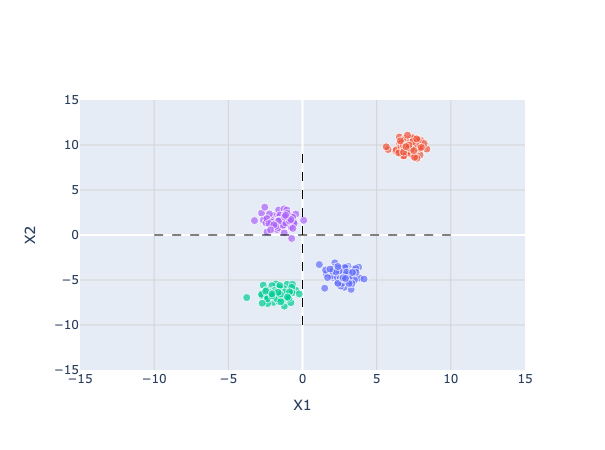
\includegraphics[width=10cm,height=10cm]{images/image1.png}
\caption{Clusters Generated}
\label{fig:clusters_generated}
\end{figure}

\subsection*{(b) K-means clustering with K = [1,2,3,4,5,6,7,8,9,10]}

With the data generated in the previous step, the K-means clustering algorithm is applied with K = [1,2,3,4,5,6,7,8,9,10]. 
The results are visualized in Figure~\ref{fig:kmeans_clustering}.

\begin{figure}[h!]
\centering
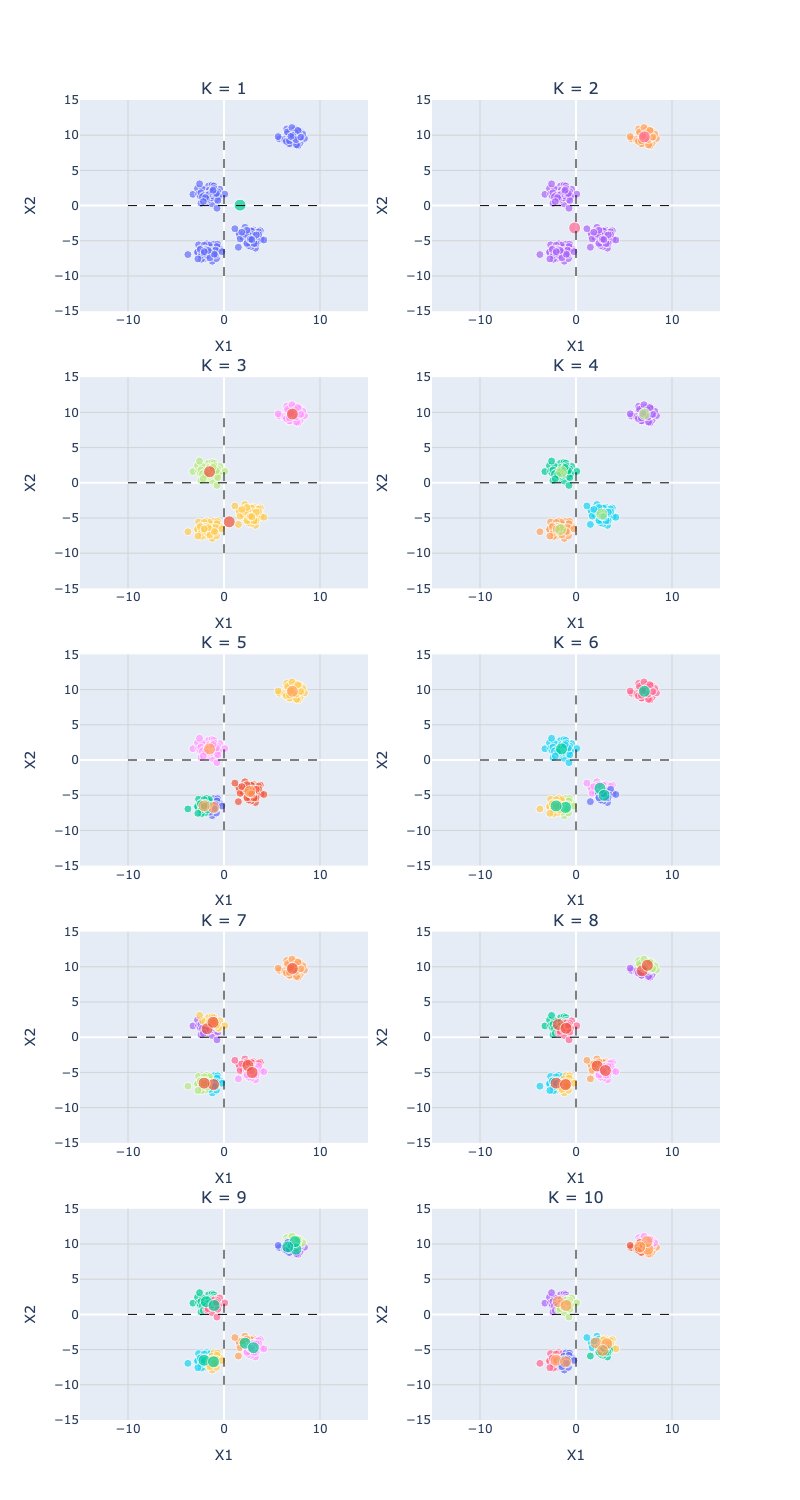
\includegraphics[width=10cm,height=20cm]{images/image2.png}
\caption{K-means Clustering}
\label{fig:kmeans_clustering}
\end{figure}

The figure shows when K $<$ 4, the centers of the clusters are not well defined with the data points generated. 
They are in the middle of all the clusters.

When K = 4, the centers provided by K-means are well positioned because the data points generated were created with 4 clusters.

When K $>$ 4, the centers provided by K-means are well positioned but it starts to create multiple centers for the same cluster.


\section*{Assignment 2}


\section*{Assignment 3}



\end{document}
